\normaltrue \difficilefalse \tdifficilefalse
\correctiontrue

%\UPSTIidClasse{11} % 11 sup, 12 spé
%\newcommand{\UPSTIidClasse}{11}

\exer{Identification $\star$ \label{B2:06:503}}
\setcounter{question}{0}\marginnote{\xpComp{SLCI}{07}}%\UPSTIcompetence[2]{B2-06}
\index{Compétence B2-06}
\index{Identification}
\index{Identification Bode}
\index{Identification fréquentielle}
\index{Réponse fréquentielle}

\ifcorrection
\else
\marginnote{\textbf{Pas de corrigé pour cet exercice.}}
\fi


\ifprof 
\else

\marginnote{D'après Florestan Mathurin.}

Soit un système dont le diagramme de Bode est donné ci-dessous.
\begin{marginfigure}
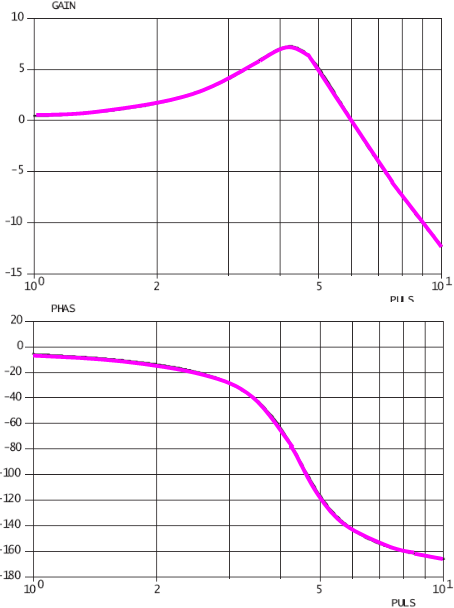
\includegraphics[width=\linewidth]{503_01}
\end{marginfigure}
\fi

\question{Tracer le diagramme de Bode asymptotique.}
\ifprof
\begin{marginfigure}
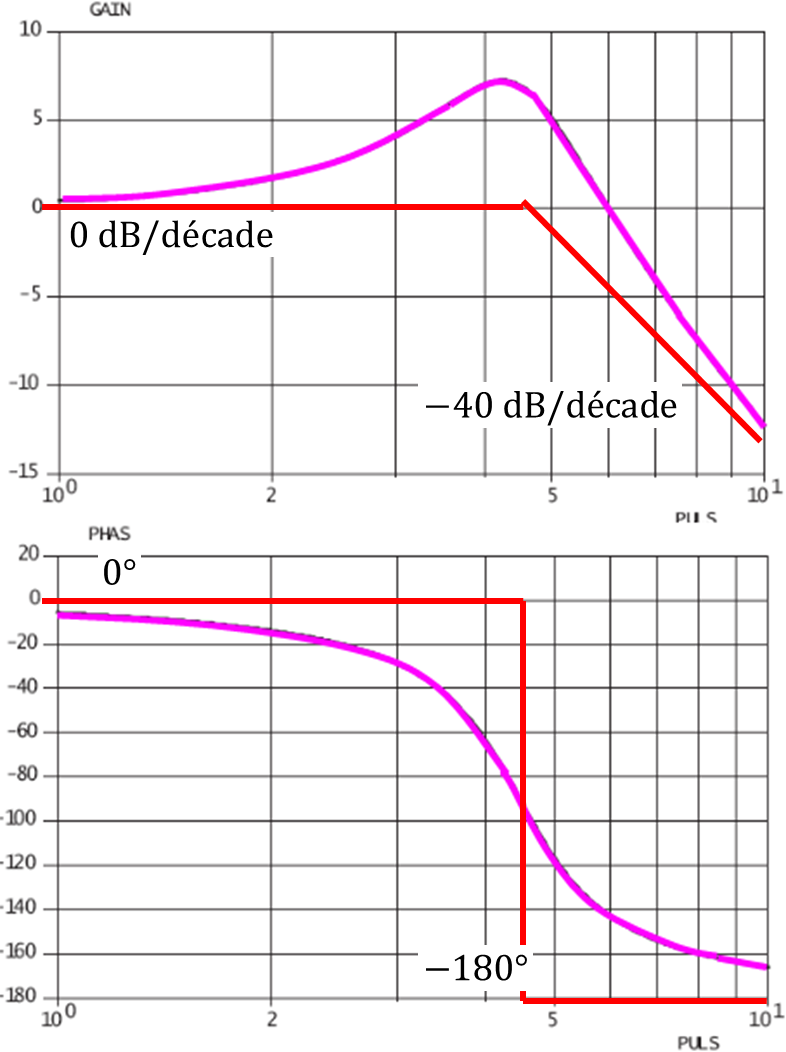
\includegraphics[width=\linewidth]{503_01_cor}
\end{marginfigure}
\else
\fi


\question{Identifier le type de la fonction de transfert et ses valeurs remarquables.}
\ifprof
La phase tend vers 0 lorsque $\omega$ tend vers \SI{0}{rad/s} et vers $-180\degres$ lorsque $\omega$ tend vers l'infini. 
On observe de plus une résonance. Par ailleurs le gain est nul quand $\omega$ tend vers \SI{0}{rad/s}. 
Le système est donc d'ordre 2 avec un gain unitaire et un $\xi<\dfrac{\sqrt{2}}{2}$. 
On détermine $\omega_0$ lorsque la phase vaut $-90\degres$.

À ce stade, $H(p)=\dfrac{1}{1+\dfrac{2\xi}{4,5}p+\dfrac{p^2}{4,5^2}}$.

Enfin, on mesure un gain à la résonance de \SI{7}{dB}. 
On a donc $20\log A_{\text{max}}=7$ soit $A_{\text{max}}=10^{7/20}= \dfrac{1}{2\xi\sqrt{1-\xi^2}}$.

Par suite, 
 $\dfrac{1}{A_{\text{max}}}=2\xi\sqrt{1-\xi^2}$
 $\Leftrightarrow \dfrac{1}{A_{\text{max}}}=4\xi^2\left(1-\xi^2\right)$
 $\Leftrightarrow \dfrac{1}{A^2_{\text{max}}}=4\xi^2-4\xi^4$
  $\Rightarrow 4\xi^4 -4\xi^2+ \dfrac{1}{A^2_{\text{max}}}=0$ 
  $\Rightarrow 4X^2 -4X+ \dfrac{1}{A^2_{\text{max}}}=0$
  
 On a alors $\Delta = 16 -  \dfrac{16}{A^2_{\text{max}}}$ et $X_{1,2} = \dfrac{4\pm\sqrt{\Delta}}{16}$
 
 En réalisant les applications numériques, on a $\xi = \sqrt{\dfrac{4-\sqrt{\Delta}}{16}} = 0,23$.
  
Alors, $H(p)=\dfrac{1}{1+\dfrac{2\times 0,23}{4,5}p+\dfrac{p^2}{4,5^2}}$.
\begin{marginfigure}
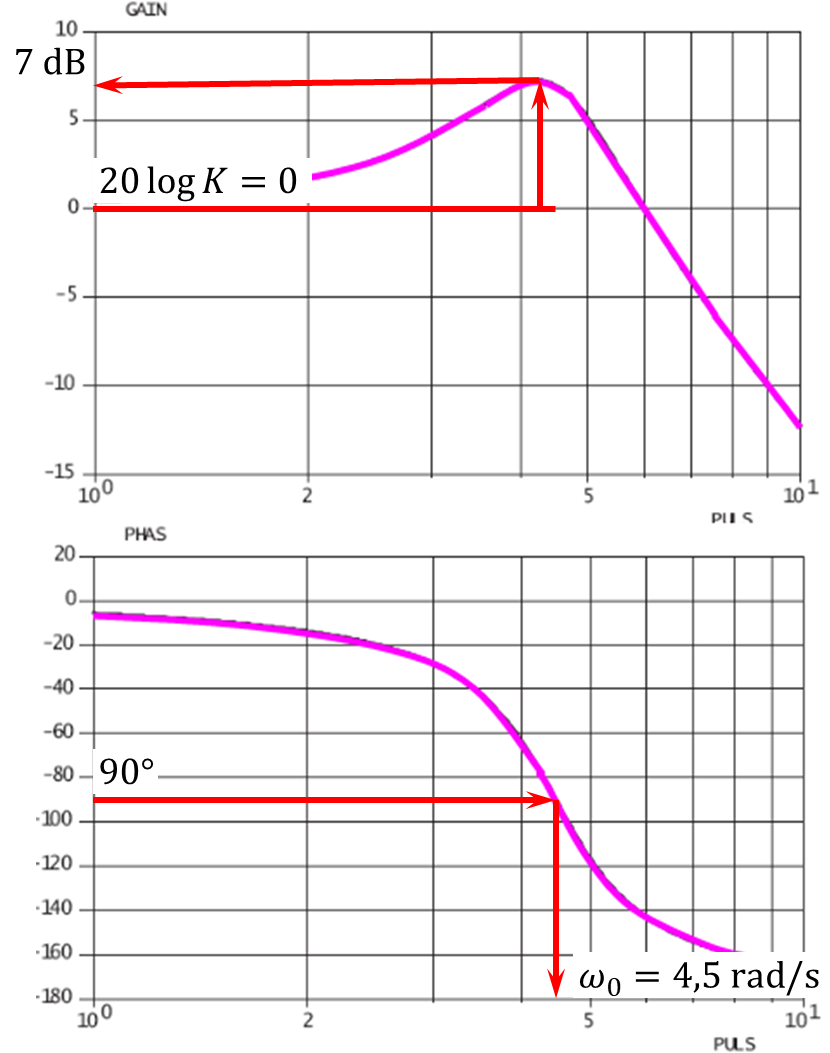
\includegraphics[width=\linewidth]{503_02_cor}
\end{marginfigure}
\else

Le diagramme temporel ci-dessous présente 3 signaux d'entrée sinusoïdaux.
\begin{marginfigure}
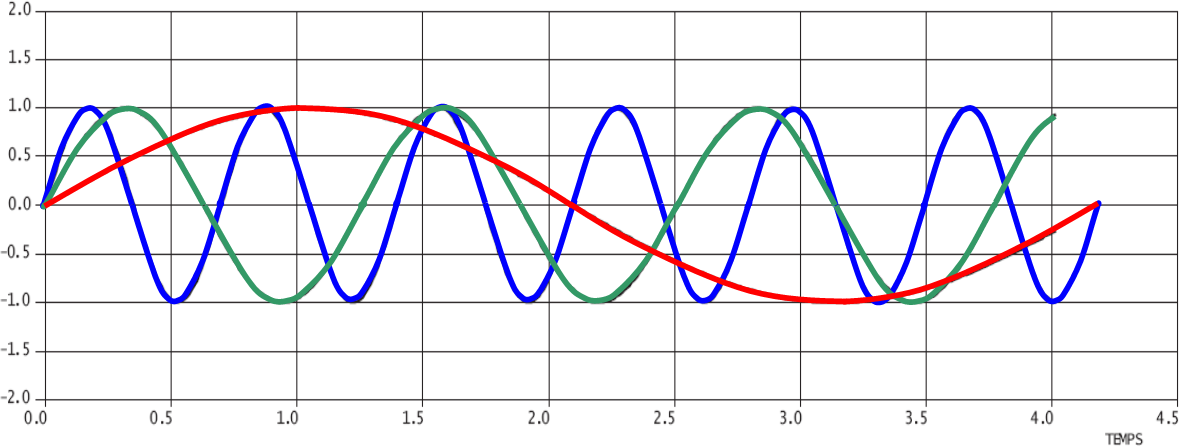
\includegraphics[width=\linewidth]{503_02}
\end{marginfigure}

\fi

\question{Déterminer les période et les pulsations de chacun des signaux.}
\ifprof
\begin{itemize}
\item Signal rouge : $T=\SI{4,2}{s}$ et $\omega= \dfrac{2\pi}{T} = \SI{1,5}{rad/s}$.
\item Signal vert : $T=3,6/3 = \SI{1,2}{s}$ et $\omega= \dfrac{2\pi}{T} = \SI{5,2}{rad/s}$.
\item Signal bleu : $T=4,2/6 = \SI{0,7}{s}$  et $\omega= \dfrac{2\pi}{T} = \SI{9}{rad/s}$.
\end{itemize}
\else
\fi


\question{En déduire le gain et le déphasage en régime permanent pour chacune des courbes temporelles de sortie correspondant aux 3 entrées.}
\ifprof
\begin{marginfigure}
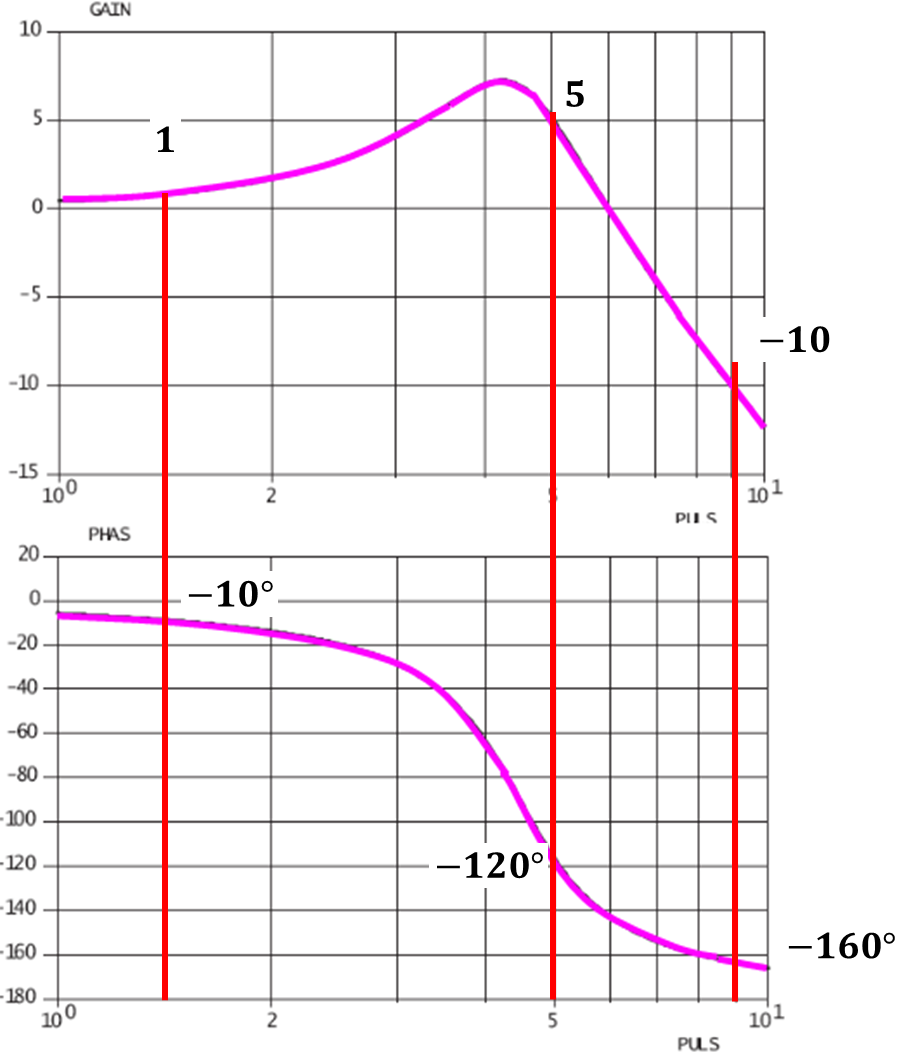
\includegraphics[width=\linewidth]{503_03_cor}
\end{marginfigure}

\begin{itemize}
\item Pour  $\omega = \SI{1,5}{rad/s}$, $G_{\text{dB}}=1 \Rightarrow 20\log K = 1 \Rightarrow  K = 10^{1/20} = 1,12$ et $\varphi =  -\SI{0,17}{rad}$. On a donc $s(t)=1,12\sin\left(\omega t - 0,17\right)$.
\item Pour  $\omega = \SI{5}{rad/s}$, $G_{\text{dB}}=5 \Rightarrow  K = 10^{5/20} = 1,8$ et $\varphi =  -\SI{2,1}{rad}$. On a donc $s(t)=1,8\sin\left(\omega t - 2,1\right)$.
\item Pour  $\omega = \SI{9}{rad/s}$ $G_{\text{dB}}=5 \Rightarrow  K = 10^{-10/20} = 0,3$ et 
$\varphi =  -\SI{2,8}{rad}$. On a donc $s(t)=0,3\sin\left(\omega t - 2,8\right)$.
\end{itemize}
\else
\fi





\ifprof
\else


\begin{solution}
\begin{enumerate}
\item .
\item $H(p)=\dfrac{1}{1+\dfrac{2\times 0,23}{4,5}p+\dfrac{p^2}{4,5^2}}$.
\item .
\begin{itemize}
\item Signal rouge : $T=\SI{4,2}{s}$ et $\omega \SI{1,5}{rad/s}$.
\item Signal vert : $T=3,6/3 = \SI{1,2}{s}$ et $\omega= \SI{5,2}{rad/s}$.
\item Signal bleu : $T=4,2/6 = \SI{0,7}{s}$  et $\omega= \SI{9}{rad/s}$.
\end{itemize}
\item .
\begin{itemize}
\item $s(t)=1,12\sin\left(\omega t - 0,17\right)$.
\item $s(t)=1,8\sin\left(\omega t - 2,1\right)$.
\item $s(t)=0,3\sin\left(\omega t - 2,8\right)$.
\end{itemize}
\end{enumerate}
\end{solution}


\marginnote{Corrigé voir \ref{B2:06:503}.}

\fi